\documentclass[12pt, letterpaper]{article}
\usepackage{graphicx}
\graphicspath{{files/img/}}
\title{VAR{title}}
\author{VAR{author}}
\date{VAR{date}}


\begin{document}
\maketitle


\section{The Graphical Plot}
\begin{figure}[h]
     \centering
    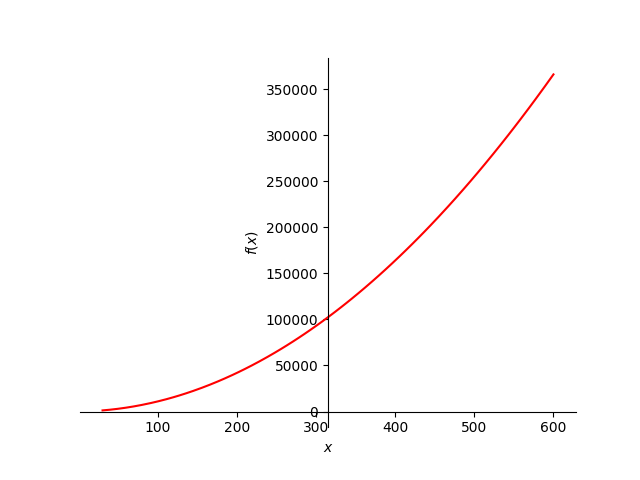
\includegraphics[width=0.75\textwidth]{simple_plot}
    \caption{A plot for $x + 2*y = 10$}
    \label{fig:simple_plot1}
\end{figure}

\newpage

\section{The HPI and PDI values}
\begin{center}

%- if renderTbl == True
\begin{tabular}{|| c  c  c  c c ||}
\hline
 Country & Nominal HPI  & Real HPI  & Nominal PDI & Real PDI \\ [0.5ex]
\hline \hline
Australia & 7.59691301221876 & 38.608650078914  & 14.6931416270543 & 74.677320989926 \\
\hline
Beligum & 15.2222569986975 & 44.5657736355528 & 22.1724332186943 & 64.8992596919942 \\
\hline
Canada & 17.4345104685643 & 64.2715168780115 & 19.8824844065116  & 73.2909435105582 \\  [1.0ex]
\hline

\end{tabular}

%- endif

%- if renderTbl == False
No tabular data available.
%- endif

\end{center}

\end{document}